\documentclass[preprint,11pt,5p,twocolumn]{elsarticle}
\usepackage[utf8]{inputenc}
\usepackage{amssymb}
\usepackage{bm}
\usepackage{mathtools}
\usepackage{xfrac}
\usepackage{graphicx}
\usepackage{caption}
\usepackage{subcaption}
\usepackage{lineno}

\usepackage[hidelinks]{hyperref}
\usepackage[nameinlink]{cleveref}

\usepackage{afterpage}

\newcommand{\matr}[1]{\mathbf{#1}}

\makeatletter
\providecommand{\doi}[1]{%
  \begingroup
    \let\bibinfo\@secondoftwo
    \urlstyle{rm}%
    \href{http://dx.doi.org/#1}{%
      doi:\discretionary{}{}{}%
      \nolinkurl{#1}%
    }%
  \endgroup
}

\let\oldhref\href
\renewcommand{\href}[2]{\oldhref{#1}{\hbox{#2}}}
\makeatother

\begin{document}

\hyphenation{Conv-LSTM}
\hyphenation{Conv-LSTMs}

\begin{frontmatter}

%% Title, authors and addresses

%% use the tnoteref command within \title for footnotes;
%% use the tnotetext command for theassociated footnote;
%% use the fnref command within \author or \address for footnotes;
%% use the fntext command for theassociated footnote;
%% use the corref command within \author for corresponding author footnotes;
%% use the cortext command for theassociated footnote;
%% use the ead command for the email address,
%% and the form \ead[url] for the home page:
%% \title{Title\tnoteref{label1}}
%% \tnotetext[label1]{}
%% \author{Name\corref{cor1}\fnref{label2}}
%% \ead{email address}
%% \ead[url]{home page}
%% \fntext[label2]{}
%% \cortext[cor1]{}
%% \address{Address\fnref{label3}}
%% \fntext[label3]{}

\title{Multi-output Bus Travel Time Prediction\\
with Convolutional LSTM Neural Networks}

\journal{Expert Systems with Applications}

%% use optional labels to link authors explicitly to addresses:
%% \author[label1,label2]{}
%% \address[label1]{}
%% \address[label2]{}

\author{Niklas Christoffer Petersen\\[.25em]\footnotesize{niklch@dtu.dk}}

\address{
  \vspace{.5em}
  \begin{minipage}{.5\textwidth}
    \center
    Department of Management Engineering \\
    Technical University of Denmark, 2800 Kongens Lyngby 
  \end{minipage}% This must go next to `\end{minipage}`
  \begin{minipage}{.5\textwidth}
    \center
    Public Transport Movia \\
    Gammel Køge Landevej 3, 2500 Valby 
  \end{minipage}
  \vspace{-2.5em}
}

\begin{abstract}
Accurate and reliable predictions for travel times in public transport networks is essential for delivering an attractive service.
This paper presents a multi-output, multi-time-step, deep neural network for bus travel time prediction using Convolutional and Long short-term memory (LSTM) layers. The method is empirically evaluated and compared to other popular approaches for link travel time prediction, and currently available services. We find that the proposed model significantly outperforms all the other methods, and is able to detect small irregular peeks in bus travel time very quickly.
\end{abstract}

\begin{keyword}
%% keywords here, in the form: keyword \sep keyword
Bus Travel Time Prediction \sep Intelligent Transport Systems \sep Convolutional Neural Network (CNN) \sep Long short-term memory (LSTM), Deep Learning.
\end{keyword}

\end{frontmatter}
\section{Introduction}
Public transport authorities have long found that GPS trajectory data from already deployed \emph{Automatic Vehicle Location}-systems (AVL) can be used in \emph{Intelligent Transport Systems} (ITS) \cite{Tcrp48}. Examples include real-time traffic information for passengers, e.g.\ smartphone travel planner apps, in-vehicle infotainment screens and departure boards. Studies has shown that reliable real-time information at bus stops has a statistical significant dampening effect on the perceived waiting time \cite{Fan2016}.

Besides real-time passenger information, robust arrival- and departure time predictions are necessary for operating more sophisticated ITS applications successfully, e.g. \emph{connection assurance} between low frequent public transport services, where accurate arrival times are needed to decide if one of the services should wait on the other. Another example is \emph{demand-adaptive transit systems}, where prolonged travel time should be taken into account because of the influence on both vehicle and driver utilization, and thus the efficiency of the transit system. Arrival/departure time prediction is commonly approached as a specialization of travel time prediction as illustrated in \Cref{fig:bus-arrival-links}. The predicted travel time for each link is simply accumulated downstream the route to yield the arrival/departure time predictions at each stop point of the rest of the current journey. Besides the link travel time, estimations of dwell time (i.e.\ when a bus is holding at a stop point) are also accumulated downstream.

\begin{figure}[!ht]
  \center  
  
\includegraphics[width=\columnwidth]{drawings/bus-arrival-links-narrow.pdf}
  \caption{Arrival- and departure using link travel time.}
  \label{fig:bus-arrival-links}
\end{figure}

Producing precise bus travel time predictions in areas with little external influence, e.g.\ rural areas, can be solved to a large extent with historical averaging or simple regression methods \cite{Williams2003,Altinkaya2013}. The problem becomes much more complex in urban areas where congestion, events, road-works, weather, etc.\ highly influence the traffic flow and passenger demand. As on-board GPS and AVL-systems has become more affordable and common, data has both grown in coverage, i.e.\ number of vehicles with AVL installed, and frequency, i.e.\ number of GPS-positions collected per vehicle.

In this paper we present a multi-output, multi-time-step deep neural network for bus travel time prediction using a combination of \emph{Convolutional} and \emph{Long short-term memory} (LSTM) \cite{Lstm1,Lstm2} layers. The goal of this work is to produce precise short-term predictions (e.g.\ $0-1.5$ hours) for link travel time, specifically for bus traffic in urban areas. The method is empirically evaluated and compared to other popular approaches for link travel time prediction, including the currently model deployed in production by the public transport authority for the Greater Copenhagen Area: \emph{Movia}. Furthermore the method is compared to Google Traffic, a popular online service for travel time prediction. 

This paper is structured in the following manner: In the next section, related work and literature are reviewed. \Cref{sec:convlstm} introduces Convolutional LSTM neural networks in general and in \Cref{sec:model} we present the proposed multi-output model in more details, including e.g.\ network topology, etc. \Cref{sec:experiments} introduces the Copenhagen-dataset, which the model has been evaluated on, and our results are presented and discussed in~\Cref{sec:results}. Finally we conclude on the work in~\Cref{sec:conclusion}.

\section{Literature review}
Bus link travel time prediction has been explored in research as GPS and AVL data has become increasingly available. The problem overlaps with other research areas such as general traffic flow and speed estimation, but also has unique constraints and opportunities that follows from servicing a fixed route. The improvement in computational power in the recent decades has gradually allowed more complex link travel time models with increased precision.

Early approaches for bus travel time prediction rely on historical averaging models \cite{Dailey1999,Sun2007}, and linear regression \cite{Patnaik2004}. Recent research presents this type of model only for comparison purposes, and the models are in all cases outperformed by the proposed models \cite{Shalaby2004,Jeong2005}. A historical averaging model will only slowly converge to changes in the travel time, which of cause is undesired with short, but highly impacting, external influences (e.g.\ a traffic incident or large event). 

Kalman-filters, which by its capabilities of maintaining state between predictions, has shown interest from several studies for capturing \emph{changes} in the travel time, either as an independent model \cite{Chen2001,Shalaby2004} or in combination with other models \cite{Yo2010,Bai2015}. The Kalman-filter models still have limited options for capturing and forecasting the complex dynamics of travel and dwell time in a metropolitan bus system. E.g., the Kalman-filter's state is only directly accessible for the leading time-step, and thus not capable of finding long-distance patterns spanning over several links and/or over several time-steps. This is substantiated by \cite{Lin2013} and \cite{Kumar2014}, who find artificial neural networks (ANN) to outperform Kalman-filter models. However, the computational challenges of fully connected ANNs is also limiting the depth of the network and thus how complex patterns it can learn to recognize. This has sparked the interest for studying composite or hybrid models. \citet{Bai2015} uses a two-stage approach by combining offline ANN-models, with an adaptable/online Kalman-filter to yield a dynamic model. The model is not actually learning in the long term, but is able to adapt to temporal variations in the current travel time on a journey, and is still not able to recognize long distance patterns. The proposed model in this work uses \emph{Long short-term memory} cells (LSTM), and differs from existing research in bus link travel time prediction by combining the capability for persisting state-space over multiple time-steps, while allowing the deep neural network to be feasibly trainable.

Some recent research recognizes that several routes can benefit from each other's predictions if they share some partial route segment, e.g.\ \cite{Yu2011,Gal2014,Bai2015}, however none of these approaches consider cross temporal correlations between different route segments, and only use a small window for correlation with upstream links (e.g.\ max.\ 3 links). Likewise, \citet{YanjieDuan2016} proposes to use a LSTM model for general highway travel time prediction, and do predict multiple time-steps ahead, but only for a single link at a time, i.e.\ cross link (spatial) correlations are lost. In contrast the combination of both \emph{LSTM} cells and \emph{Convolutional} filters for bus travel time prediction, proposed in this paper, allows the learned patterns to generalize beyond a single link and time, i.e.\ multi-output and multi-time-step. Furthermore this reduces the computational complexity by magnitudes compared to fully connected ANNs capable of capturing similar complex patterns.

\section{Convolutional LSTM neural networks}
\label{sec:convlstm}
A Long short-term memory (LSTM) neural network is a special type of Recurrent Neural Network~(RNN) which has proven robust for capturing long-distance dependencies \cite{Lstm1,Lstm2}. The important feature of a LSTM network is its capability to persist cell state, $\matr{c}_t$, from previous observations across sequences of input (e.g.\ time), but also eliminate information which is considered irrelevant. To allow this mechanism the persistence of information is controlled by three gates: \emph{input gate}, \emph{forget gate}, and \emph{output gate}. Each gate yields a state value at time $t$, respectively $\matr{i}_t$, $\matr{f}_t$, and $\matr{o}_t$, along with the cell output, $\matr{h}_t$, cf.~\cref{eq:lstm}, where $\circ$ denotes the entry-wise product.

\begin{equation}
\begin{aligned}
  \matr{i}_t &= \sigma \left( \matr{W}^i \matr{x}_t + \matr{R}^i \matr{h}_{t-1} + \matr{U}^i \circ \matr{c}_{t-1} + \matr{b}^i \right) \\
  \matr{f}_t &= \sigma \left( \matr{W}^f \matr{x}_t + \matr{R}^f \matr{h}_{t-1} + \matr{U}^f \circ \matr{c}_{t-1} + \matr{b}^f \right) \\
  \matr{c}_t &= \matr{f}_t \circ \matr{c}_{t-1} + \matr{i}_t \circ \mathrm{tanh} \left( \matr{W}^c \matr{x}_t + \matr{R}^c \matr{h}_{t-1} + \matr{b}_c \right) \\
  \matr{o}_t &= \sigma \left( \matr{W}^\mathit{o} \matr{x}_t + \matr{R}^\mathit{o} \matr{h}_{t-1} + \matr{U}^\mathit{o} \circ \matr{c}_{t} + \matr{b}^o \right) \\
  \matr{h}_t &= \matr{o}_t \circ \mathrm{tanh} \left( \matr{c}_t \right)
\end{aligned}
\label{eq:lstm}
\end{equation}
\vspace{.5em}

\Cref{fig:lstm-peepholes} illustrates the inner structure of a LSTM cell with peephole as proposed by \cite{LstmPeephole}. 
Is has especially grown popular for predicting time series using methods evolved from \cite{LstmTs}, where fixed-length windows of time-series are generated and feed into a LSTM network. Multiple LSTMs can be stacked such that more complex patterns of sequential information (e.g.\ temporal patterns) can be learned.

\begin{figure}[!ht]
  \centering
  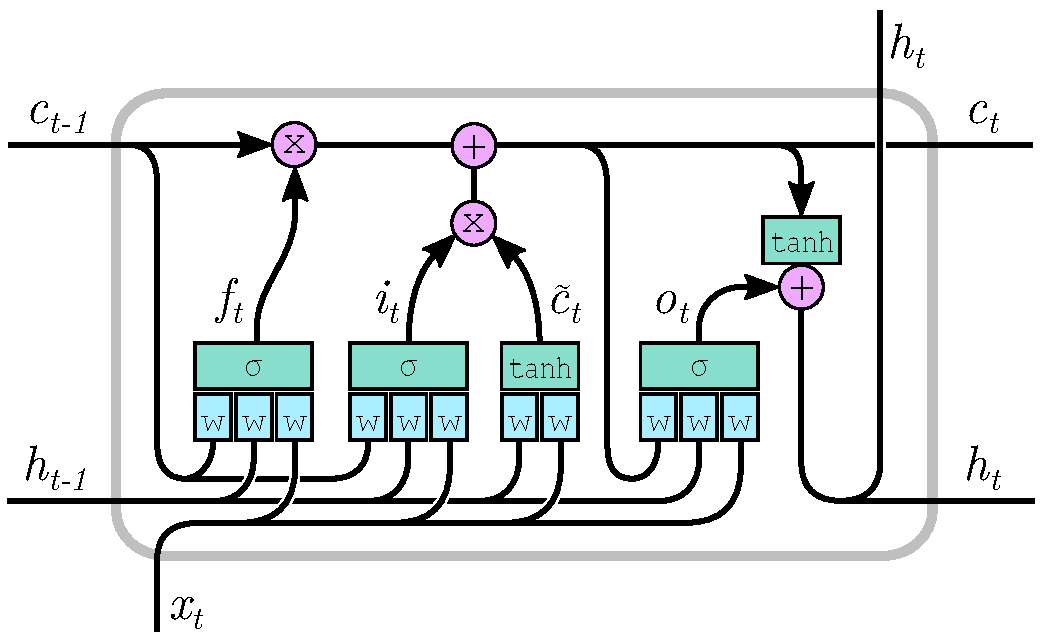
\includegraphics[scale=.45]{drawings/lstm-peepholes.pdf}
  \caption{Structure of LSTM cell with peephole.}
  \label{fig:lstm-peepholes}
\end{figure}

Convolutional Neural Networks~(CNN) on the other hand have been widely used for capturing spacial relationships, e.g.\ importance of neighboring pixels in an image. As opposed to fully connected layers, where each unit, $i$, in the layer, has a dedicated scalar weight, $w_{ij}$, for all input value, $x_j$, convolutional units are only locally connected and reuse the same weights for producing several outputs. Instead of considering the entire input-vector, only a fixed-size window, or \emph{convolution}, around each input is considered. The weights are therefore referred to as the \emph{filters} or \emph{kernels} of the layer. \Cref{fig:conv} illustrates a single convolutional filter of size $3$ being applied to 1-dimensional data.

\begin{figure}[!ht]
  \centering
  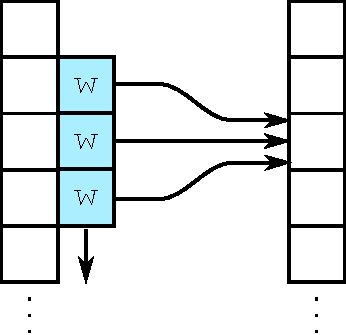
\includegraphics[scale=.45]{drawings/conv.pdf}
  \caption{Application of Convolutional filter onto 1D data.}
  \label{fig:conv}
\end{figure}

Special care needs to be taken on the boundaries, i.e.\ where the convolutional filter will exceed the input. A popular approach to avoid the size of the output decreases is to pad the input, e.g.\ with zeros. This ensures that the output shape of each convolutional unit will always be identical to the input shape, which is often desirable. One of the key benefits of convolutional networks is that the number of weights that needs to be learned is considerably reduced compared to fully connected networks, and that learned patterns can be transfered across space. I.e.\ the convolutional filters become feature detectors, that in our case can detect spatial patterns across links, e.g.\ congestion forming, etc.   

\citet{ConvLSTM} introduced the novel combination of Convolutional and LSTM layers into a single structure, the \emph{Convolutional LSTM}, or simply \emph{ConvLSTM}. Specifically the method applies convolutional filters in the \emph{input-to-state} and \emph{state-to-state} transitions of the LSTM cf.~\cref{eq:convlstm}, where $*$ denotes the convolution operator.
\begin{equation}
\begin{aligned}
  \matr{i}_t &= \sigma \left( \matr{W}^i * \matr{x}_t + \matr{R}^i * \matr{h}_{t-1} + \matr{U}^i \circ \matr{c}_{t-1} + \matr{b}^i \right) \\
  \matr{f}_t &= \sigma \left( \matr{W}^f * \matr{x}_t + \matr{R}^f * \matr{h}_{t-1} + \matr{U}^f \circ \matr{c}_{t-1} + \matr{b}^f \right) \\
  \matr{c}_t &= \matr{f}_t \circ \matr{c}_{t-1} + \matr{i}_t \circ \mathrm{tanh} \left( \matr{W}^c * \matr{x}_t + \matr{R}^c * \matr{h}_{t-1} + \matr{b}_c \right) \\
  \matr{o}_t &= \sigma \left( \matr{W}^\mathit{o} * \matr{x}_t + \matr{R}^\mathit{o} * \matr{h}_{t-1} + \matr{U}^\mathit{o} \circ \matr{c}_{t} + \matr{b}^o \right) \\
  \matr{h}_t &= \matr{o}_t \circ \mathrm{tanh} \left( \matr{c}_t \right)
\end{aligned}
\label{eq:convlstm}
\end{equation}
\vspace{.5em}

\begin{figure*}[!t]
  \centering
  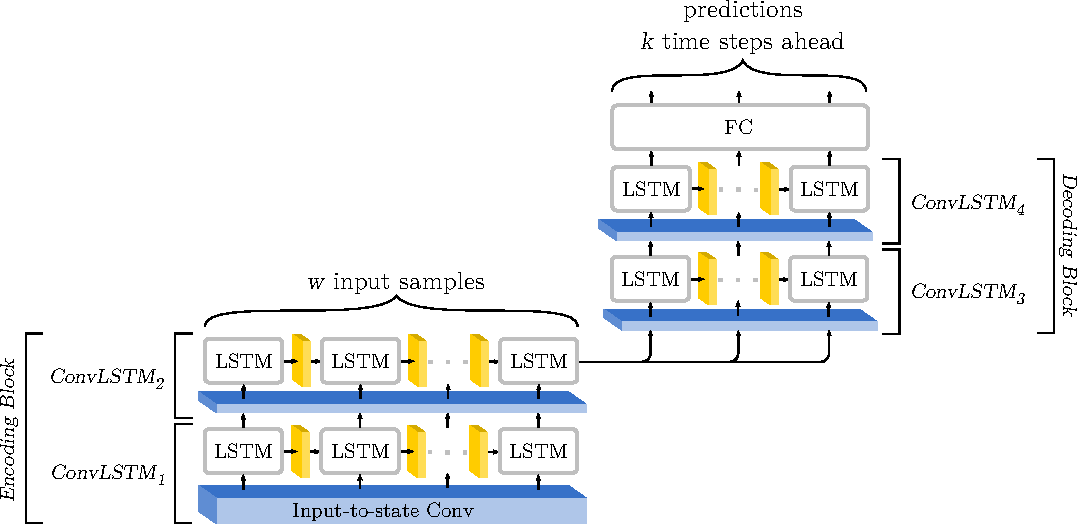
\includegraphics[scale=.75]{drawings/conv_lstm.pdf}
  \caption{Convolutional LSTM network topology.}
  \label{fig:ConvLSTM}
\end{figure*}

The output dimensionality of a \emph{ConvLSTM} layer is like the traditional CNN-layer determined by the number of filters applied. However, \emph{ConvLSTMs} require a total of eight filters for each desired output, i.e.\ four \emph{input-to-state} filters ($\matr{W}^i$, $\matr{W}^f$, $\matr{W}^c$, and $\matr{W}^o$) and four \emph{state-to-state} filters ($\matr{R}^i$, $\matr{R}^f$, $\matr{R}^c$, and $\matr{R}^o$).
Still it is important to emphasize that application of convolutional filters to the LSTM model greatly reduces the number of weights that needs to be learned, compared to a \emph{pure LSTM} approach. This allows for even deeper networks.
\newpage

\section{Multi-output model}
\label{sec:model}
In this section we present the multi-output, multi-time-step model for bus travel time prediction, which uses the \emph{ConvLSTM} introduced in the previous section.

\subsection{Network topology}


\Cref{fig:ConvLSTM} shows the overall network topology, where blue boxes illustrates \emph{input-to-state} convolutions and yellow \emph{state-to-state} convolutions. The network uses an encoder/decoder technique that to a large extent follows \cite{ConvLSTM}, where the encoder-block consists of two \emph{ConvLSTM} layers. The result is fed into a decoder, or prediction block, also consisting of two \emph{ConvLSTM} layers. The architecture allows unequal $w$ and $k$, e.g.\ predict the next $3$ time-steps based on a window size of $20$.

Thus convolutional filters are applied to each input, at each time-step, to the respective LSTM-cell, and also between LSTM-cells in the state-transition. Since the time-steps are one-dimensional~(i.e.\ link travel times across links), the filters are also one-dimensional. In each of the two blocks, the \emph{ConvLSTMs} are arranged with filter sizes of respectively $10\times1$ and $5\times1$ for each of the layers in the block. This size is used both for the \emph{input-to-state} and \emph{state-to-state} convolutional filters. Finally each \emph{ConvLSTM} layer 64~outputs, yielding a total of 512 convolutional filters.

To avoid over-fitting during training \emph{Dropout} \cite{Dropout} is performed between the \emph{ConvLSTM} layers, and \emph{Batch Normalization} \cite{BatchNorm} is also performed before each \emph{ConvLSTM} layer to ensure reasonable inputs for the activations. The dropout probability is adjusted to respectively 20\%, 10\% and 10\%.

Each of the \emph{ConvLSTM} layers uses linear activation functions, and the output from the last layer in the decoder-block is fed into a fully connected (FC) layer using the \emph{ReLU} activation function, which also ensures that only positive travel times are predicted.

\subsection{Data preparation}
We expect link travel times from AVL-systems to be available in a tabular form, where each link travel time measurement has a timestamp, and a reference to the link as illustrated in~\Cref{tab:data}.
\begin{table}[!ht]
  \centering
  \footnotesize
  \begin{tabular}{llr}
    Timestamp & Linkref. & Link travel time (s) \\ \hline \hline
    2017-10-10 00:20:02 & 29848:1254 & 63 \\ \hline
    2017-10-10 00:21:07 & 1254:1255  & 65 \\ \hline
    2017-10-10 00:21:51 & 1255:10115 & 44 \\ \hline
    \vdots & \vdots & \vdots 
  \end{tabular}
  \caption{Example of raw travel time measurements.}
  \label{tab:data}
\end{table}

For the \emph{ConvLSTM} model to be able to capture the desired spatial-–temporal patterns, the input data must be arranged in a suitable manner: I.e.\ in $N$ samples, each with a window of the $w$ lagging time-steps $t-w+1, \ldots, t$, and each time-step with $u$ link travel times $1, \ldots, u$ cf.~\Cref{fig:data_shape}.

Likewise, the output is arranged with $N$ predictions of $k$ time steps ahead, $t+1, \ldots, t+k$. Thus the input is a 4D-tensor, $\matr{X}$ with dimensionality $N \times w \times u \times 1$, and the output, $\matr{Y}$, a 4D-tensor with dimensionality $N \times k \times u \times 1$ -- in both cases the last one refers to the single link travel time for each time-step/link combination. It is emphasized that each prediction consists of travel time predictions for all links for the next $k$ time-steps, i.e.\ multi-output, multi-time-step prediction.

The $N$ samples are sampled at a fixed time resolution, since we need a shared time reference across all links. \Cref{sec:experiments} elaborates on some of the considerations for choosing a sound resolution.

\begin{figure}[!ht]
  \centering
  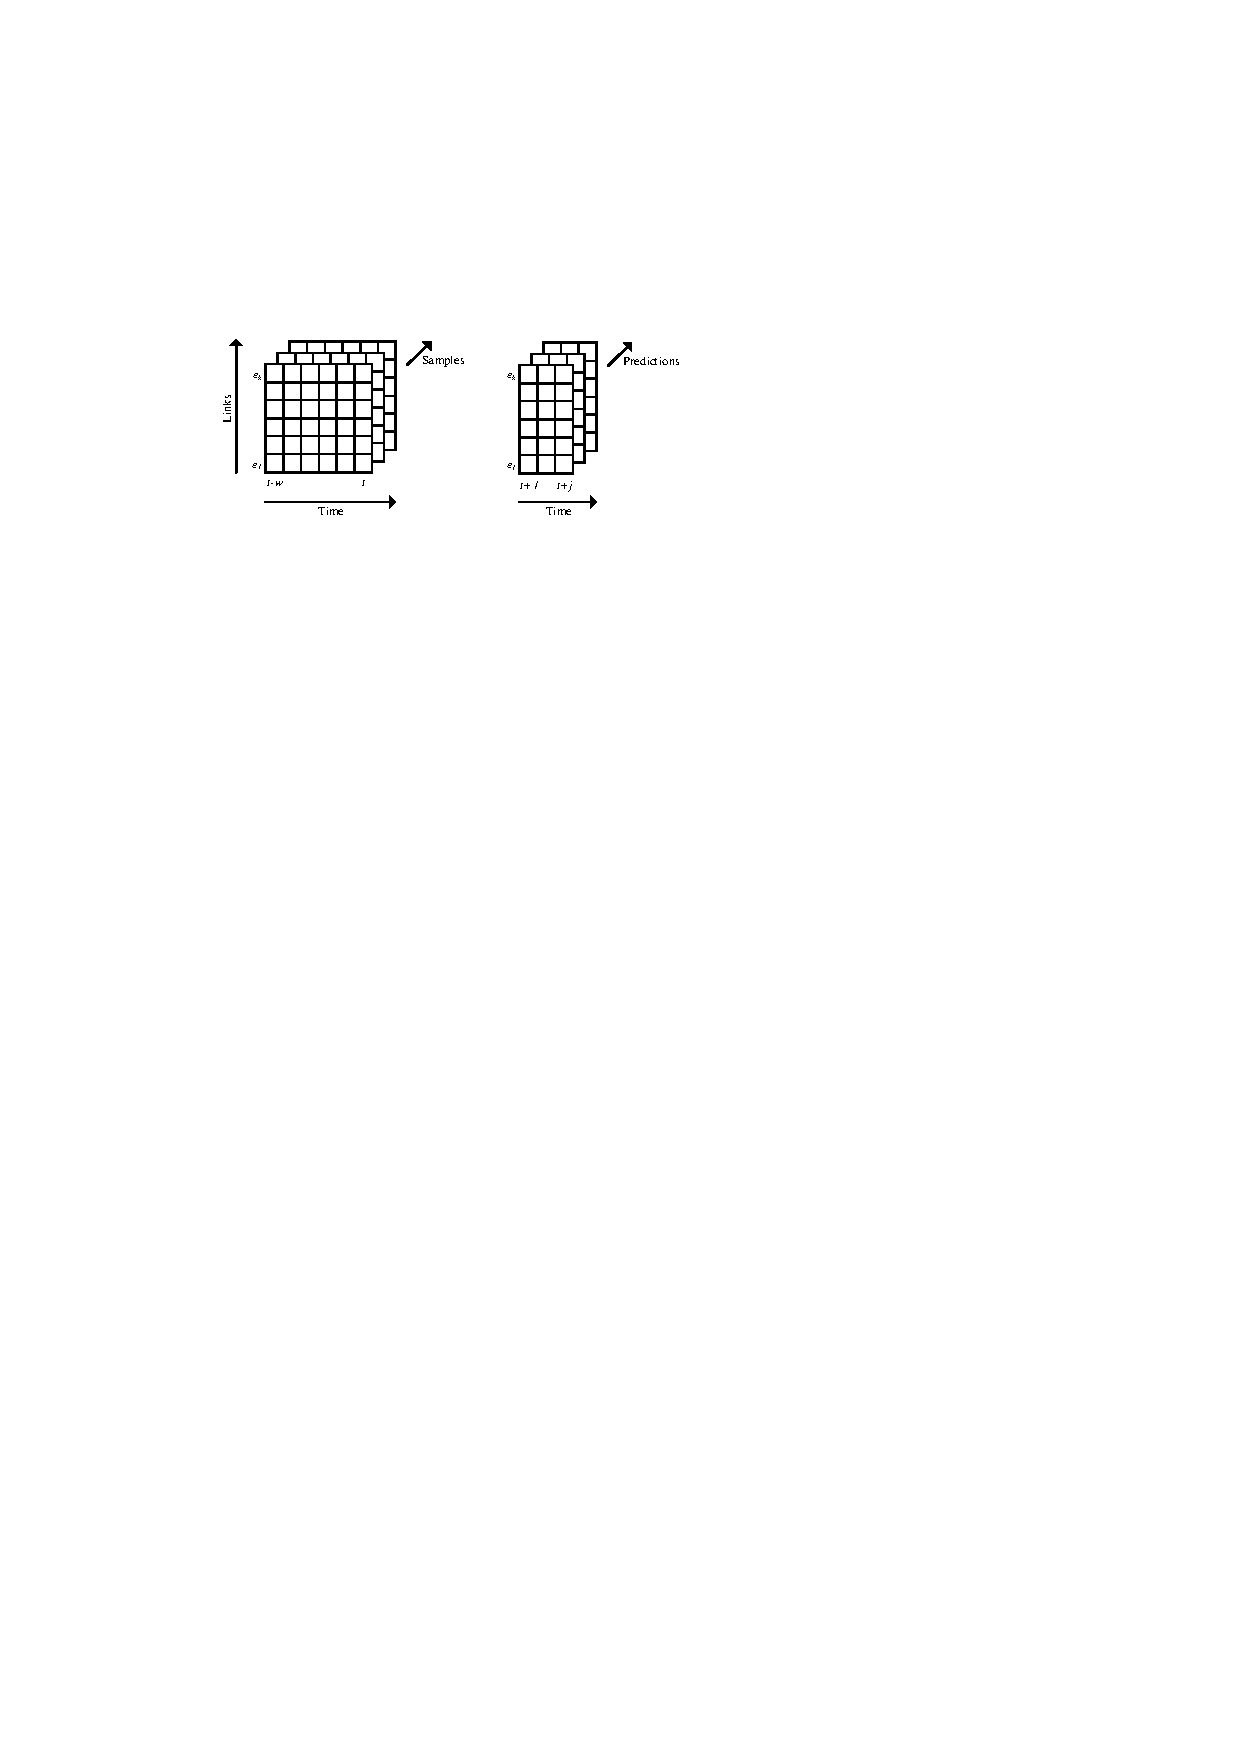
\includegraphics[scale=1.0]{drawings/data_shape.pdf}
  \caption{Shapes of the input and output data.}
  \label{fig:data_shape}
\end{figure}

\subsection{Detrending}
Urban bus travel times vary throughout the time of the day, and the day of the week due to \emph{recurring congestion}. In order to reduce the need for the network to learn this recurring variation, link travel for link $\mathit{ln} \in \{ 1,\ldots,u\}$, at time-step $t$, $x_{\mathit{ln},t}$, is normalized to focus on deviations from the normal and expected pattern. Travel times are centered with the mean for each link, at the time of day, and day of week, $\mathit{\bar{x}_{\mathit{ln},\mathit{dow},\mathit{tod}}}$, and scaled with the standard deviation for each link, $\sigma_\mathit{ln}$, cf.~\cref{eq:normalization}.

\begin{equation}
  x'_{\mathit{ln},t} = \frac{x_{\mathit{ln},t} - \bar{x}_{\mathit{ln},\mathit{dow},\mathit{tod}}}{\sigma_\mathit{ln}}
  \label{eq:normalization}
\end{equation}

A similar normalization is applied to the predicted travel times, $y_{\mathit{ln},t}$, but only using the historical mean and standard deviation, since the true mean and standard deviation obviously is unavailable in real-time prediction scenarios.

When calculating the mean and standard deviation it can be beneficial to exclude extreme outliers, since both mean and standard deviation are highly sensitive to such measurements. A suggested method is to apply \emph{absolute deviation around the median} (MAD) cf.~\cite{Olewuezi2011} when calculating $\mathit{\bar{x}_{\mathit{ln},\mathit{dow},\mathit{tod}}}$ and $\sigma_\mathit{ln}$.


\subsection{Implementation and training}
The proposed network model was implemented in Python using the Keras Framework \cite{Keras}, and trained using the \emph{RMSprop}-algorithm \cite{RMSprop}.

During training the variables $\mathit{\bar{x}_{\mathit{ln},\mathit{dow},\mathit{tod}}}$ and $\sigma_\mathit{ln}$ should be calculated solely based on the training set, to emulate the real-world application.

\section{Experiments}
\label{sec:experiments}

For the purpose of evaluation, the proposed method is applied to a dataset from Copenhagen's public transport authority: \emph{Movia}. The dataset consists of 1,2~M~travel time observations for the ``4A'' bus line in the period May to October 2017. The data points were collected using the real-time AVL-system installed in every vehicle servicing the line. 

\begin{figure}[!ht]
  \centering
  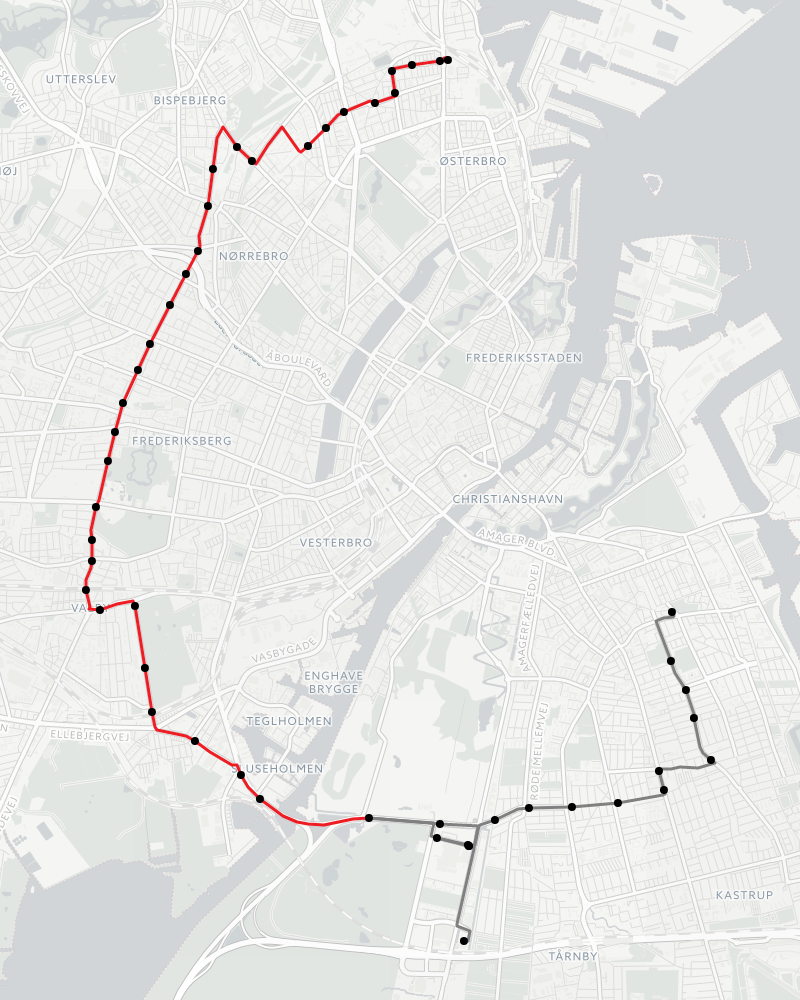
\includegraphics[width=0.4\textwidth]{drawings/map.png}
  \caption{Geography of the 4A bus line in Copenhagen.}
  \label{fig:4a_map}
\end{figure}

The geography of the route is shown in \Cref{fig:4a_map}. As the line circles Central Copenhagen, it is potentially highly sensitive to congestion to/from the city as it intersects with several large corridors along its route. Southeast of the city center the line splits in different destination patterns (gray), therefore only the first 32 links are considered in this experiment (red).


\begin{figure*}[!t]
    \centering
    \begin{subfigure}[t]{0.31\textwidth}
        \centering
        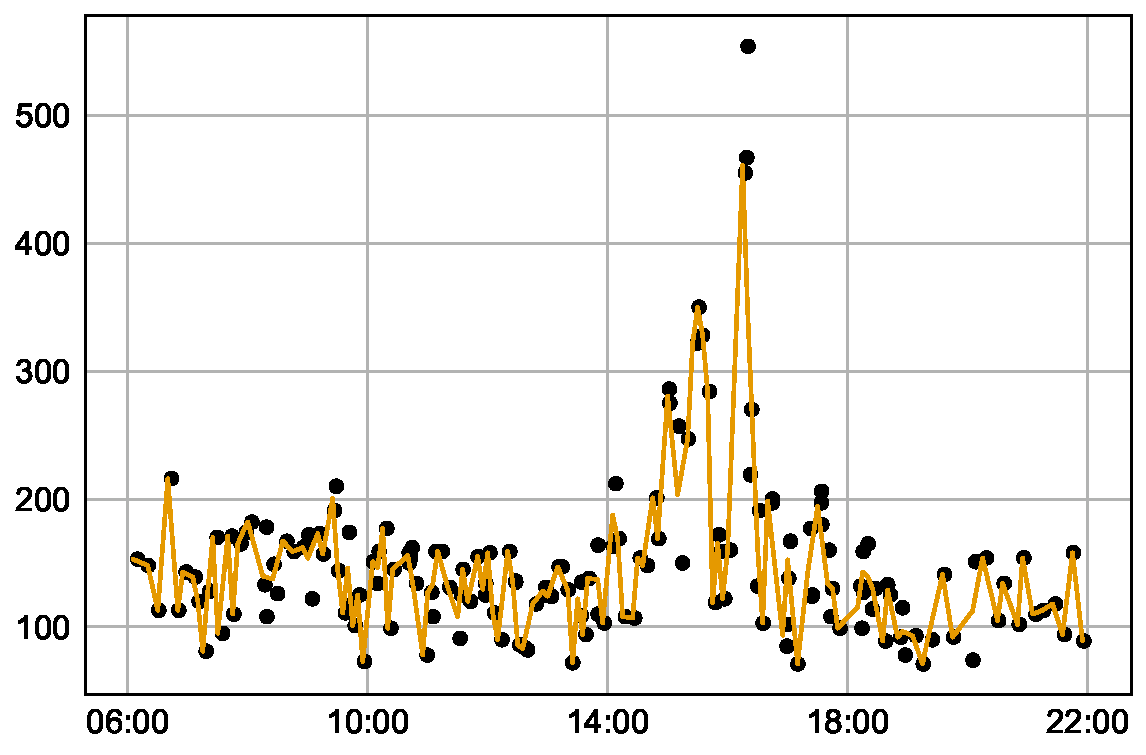
\includegraphics[width=\textwidth]{plots/decycle_5min_n.pdf}
        \caption{5 min}
    \end{subfigure}%
    ~ 
    \begin{subfigure}[t]{0.31\textwidth}
        \centering
        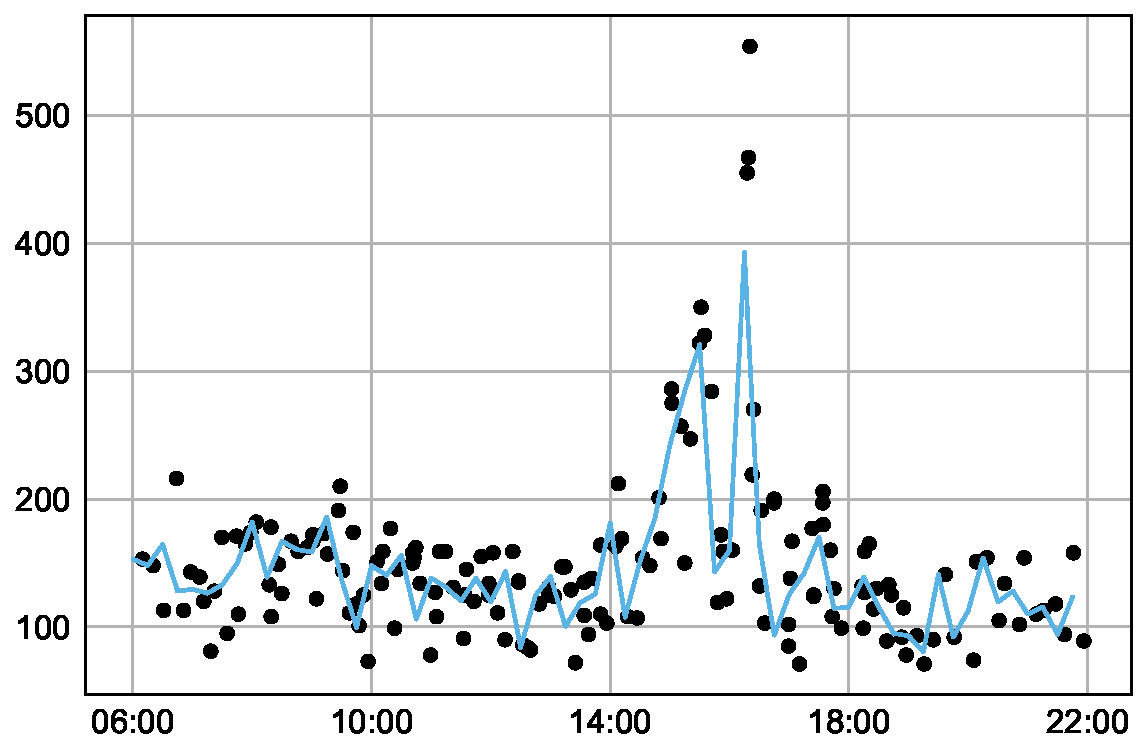
\includegraphics[width=\textwidth]{plots/decycle_15min_n.pdf}
        \caption{15 min}
    \end{subfigure}
    ~
    \begin{subfigure}[t]{0.31\textwidth}
        \centering
        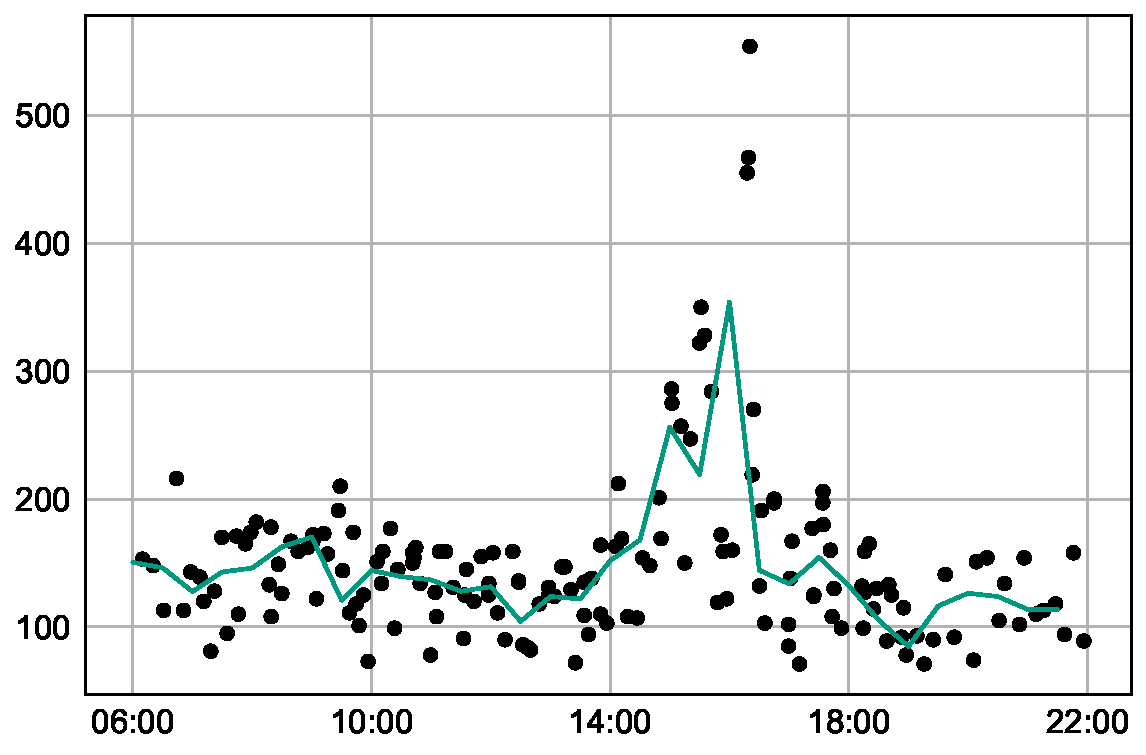
\includegraphics[width=\textwidth]{plots/decycle_30min_n.pdf}
        \caption{30 min}
    \end{subfigure}

    \caption{Examples of travel time for a single link over a single day, at various time resolutions.}
    \label{fig:resolutions}
\end{figure*}

\subsection{Time resolution}
To allow predictions for fixed time-steps ahead, data is aggregated at a fixed time resolution. \Cref{fig:resolutions} shows examples of travel time for a single link over a single day at various time resolutions. The black dots are actual measurements, and the lines the aggregated mean link travel time at the given resolution. The choice depends of the \emph{expected} frequency of the line, and is a balance between capturing the details and still having a reasonable number of measurements of each time-step to avoid over-fitting.

For this experiment data was aggregated into 15-minute time-steps and normalized cf.~\Cref{sec:model}. This resolution was chosen based on a measured mean \emph{headway} of $7.5$ minutes between 06:00 and 22:00, i.e.\ the time between two vehicles during daytime.

Given the time resolution, we set the fixed windows size, $w = 32$, equivalent of 8 hours, to allow pattern in the morning peek affect patterns in the afternoon peek. We set $k = 3$ to allow predictions of up to 45 minutes into the future. 

\subsection{Evaluation}
In order to evaluate the proposed model and comparisons, the following measures are used: \emph{mean absolute error} (MAE), \emph{root mean square error} (RMSE), and \emph{mean absolute percentage error} (MAPE) cf.~\cref{eq:mae,eq:rmse,eq:mape}, where $\matr{Y}_i$ is the true link travel times for sample $i$ and $\matr{\widehat{Y}}_i$ is the predicted travel times. Since the multi-output, multi-time-step model predicts link travel times for all $u$ links for the next $k$ time steps, $\matr{Y}_i$ and $\matr{\widehat{Y}}_i$ have both the dimensionality $w \times u \times 1$.

\begin{equation}
    \textrm{MAE}(\matr{Y}, \matr{\widehat{Y}}) = \frac{\sum_{i = 1}^{N} \left| \matr{Y}_i - \matr{\widehat{Y}}_i \right| }{N}
    \label{eq:mae}
\end{equation}

\begin{equation}
    \textrm{RMSE}(\matr{Y}, \matr{\widehat{Y}}) = \sqrt{\frac{\sum_{i = 1}^{N} \left(\matr{Y}_i - \matr{\widehat{Y}}_i \right)^2}{N}}
    \label{eq:rmse}
\end{equation}

\begin{equation}
    \textrm{MAPE}(\matr{Y}, \matr{\widehat{Y}}) = \frac{1}{N} \sum_{i = 1}^{N} \left| \frac{\matr{Y}_i - \matr{\widehat{Y}}_i}{\matr{Y}_i} \right| 
    \label{eq:mape} 
\end{equation}
\vspace{.5em}

\begin{table*}[!t]
    \center
    \begin{tabular}{ll|rrr}
        Model & Time ahead & RMSE (min) & MAE (min) & MAPE (\%) \\
        \hline         
        \hline
        Historical average &                & 4.35 & 3.23 & 6.51 \% \\ 
        \hline 
        Current model      & t + 1 (15 min) & 4.92 & 3.90 & 8.05 \% \\
                           & t + 2 (30 min) & 4.91 & 3.46 & 6.82 \% \\
                           & t + 3 (45 min) & 5.47 & 4.15 & 8.68 \% \\
        \hline 
        Pure LSTM          & t + 1 (15 min) & 3.48 & 2.48 & 5.02 \% \\
                           & t + 2 (30 min) & 3.56 & 2.51 & 5.08 \% \\
                           & t + 3 (45 min) & 3.68 & 2.62 & 5.34 \% \\
        \hline 
        Google Traffic     & t + 1 (15 min) & 3.67 & 2.96 & 6.32 \% \\ 
        \hline 
        ConvLSTM           & t + 1 (15 min) & 2.66 & 1.99 & 4.19 \% \\
                           & t + 2 (30 min) & 2.89 & 2.11 & 4.44 \% \\
                           & t + 3 (45 min) & 3.11 & 2.27 & 4.75 \% \\
        \hline 
    \end{tabular}
    \caption{Results of the proposed and the baseline models}
    \label{tab:results}
\end{table*}

To allow a clear comparison, we reduce $\matr{Y}_i$ and $\matr{\widehat{Y}}_i$ by summing over all links cf.~\cref{eq:total}. This is equivalent of predicting the total travel time of all 32 links, and follows the initial approach for arrival/departure time prediction by accumulating link travel times.
\begin{align}
    \matr{Y}_i' = \sum_{\mathit{ln} = 1}^{u} \matr{Y}_{i,\mathit{ln}} & & \matr{\widehat{Y}}_i' = \sum_{\mathit{ln} = 1}^{u} \matr{\widehat{Y}}_{i,\mathit{ln}}
    \label{eq:total} 
\end{align}

The output of each of the evaluation functions is thus simply vector of size $k$, i.e.\ the evaluation of the different time steps for all links accumulated.

The model is trained on the prepared data using a sliding window approach to simulate real-world conditions where real-time travel time measurements arrives as a continuously data stream. We use 23 weeks of data for training, and one week of data for testing.

\section{Results and discussion}
\label{sec:results}
The performance of our proposed model, based on \emph{ConvLSTM}, for link travel time prediction is compared against several other baseline models and services using the presented evaluation:
\begin{enumerate}
   \item a naïve historical average model, i.e.\ equivalent of just predicting the normalized value, $\bar{x}_{\mathit{ln},\mathit{dow},\mathit{tod}}$ 
   \item the current traffic prediction model currently deployed by Movia.
   \item a pure LSTM-model for link travel time prediction, i.e.\ without applying convolutional filters in state transitions.
   \item travel time predictions from Google Traffic (part of Google Maps).
\end{enumerate}

\Cref{tab:results} shows the overall performance of the proposed and the baseline models. Predictions are limited to daytime, i.e.\ between 06:00 and 22:00 and accumulated downstream on a journey level to simulate the use for real-time bus arrival/departure time prediction cf~\cref{eq:total}. 

Before going into a direct comparison, it is important to understand some aspects of the baseline models, and how measurements were collected.

\subsection{Historical average}
The performance of the historical average is independent with respect to the number of time steps ahead it predicts, as it just represents a weekly cycle of mean link travel times.

\subsection{Current model}
Measurements for the currently deployed bus prediction model were collected at a 5-minute frequency using a non-publicly accessible endpoint at the transport authority. The model is based on an historical average model, but has rule based mechanism on top, which can override or adjust the historical link travel times. For instance it will assume that a delayed vehicle can recover (partially or completely) from its delay by traversing links faster. Of course such an assumption can be problematic in an urban area with lots of external traffic effects. 

\subsection{Pure LSTM}
The pure LSTM-model for link travel time prediction is similar to the model proposed by \citet{YanjieDuan2016}. The model was trained on the exact same dataset as the \emph{ConvLSTM} model, and has a similar architecture, but without the convolutional filters.

\subsection{Google Traffic}
Measurements from the Google Traffic model were collected using the Google Maps Distance Matrix API~\citep{GMaps_DistanceMatrixAPI}. Google uses crowd-sourced road congestion data collected from smart-phones with the \emph{Google Maps App} installed \citep{GMaps_Crowdsourcing}. While the exact model powering the service is not publicly described in detail, the documentation states that ``that the returned \emph{duration in traffic} should be the best estimate of travel time given what is known about both historical traffic conditions and live traffic''. And further, ``that live traffic becomes more important the closer the departure time is to now'' \citep{GMaps_DistanceMatrixAPI}.

Because there is a limit on the number of requests that one freely can make to the API over a 24-hour period, it has only been possible to collect link travel times for the $t + 1$ time step (i.e.\ next 15 minutes). Travel times for each link were collected at a 15-minute interval between 06:00 and 22:00.

Another important aspect is that the Google Traffic model is primary designed for estimating car travel times, and can thus be biased away from the bus travel times used in this experiment. Since we only consider link travel time, and collection data for each link individually, the bus dwell time will not be an issue, as it is not included in either measurement.

\begin{figure*}
  \centering
  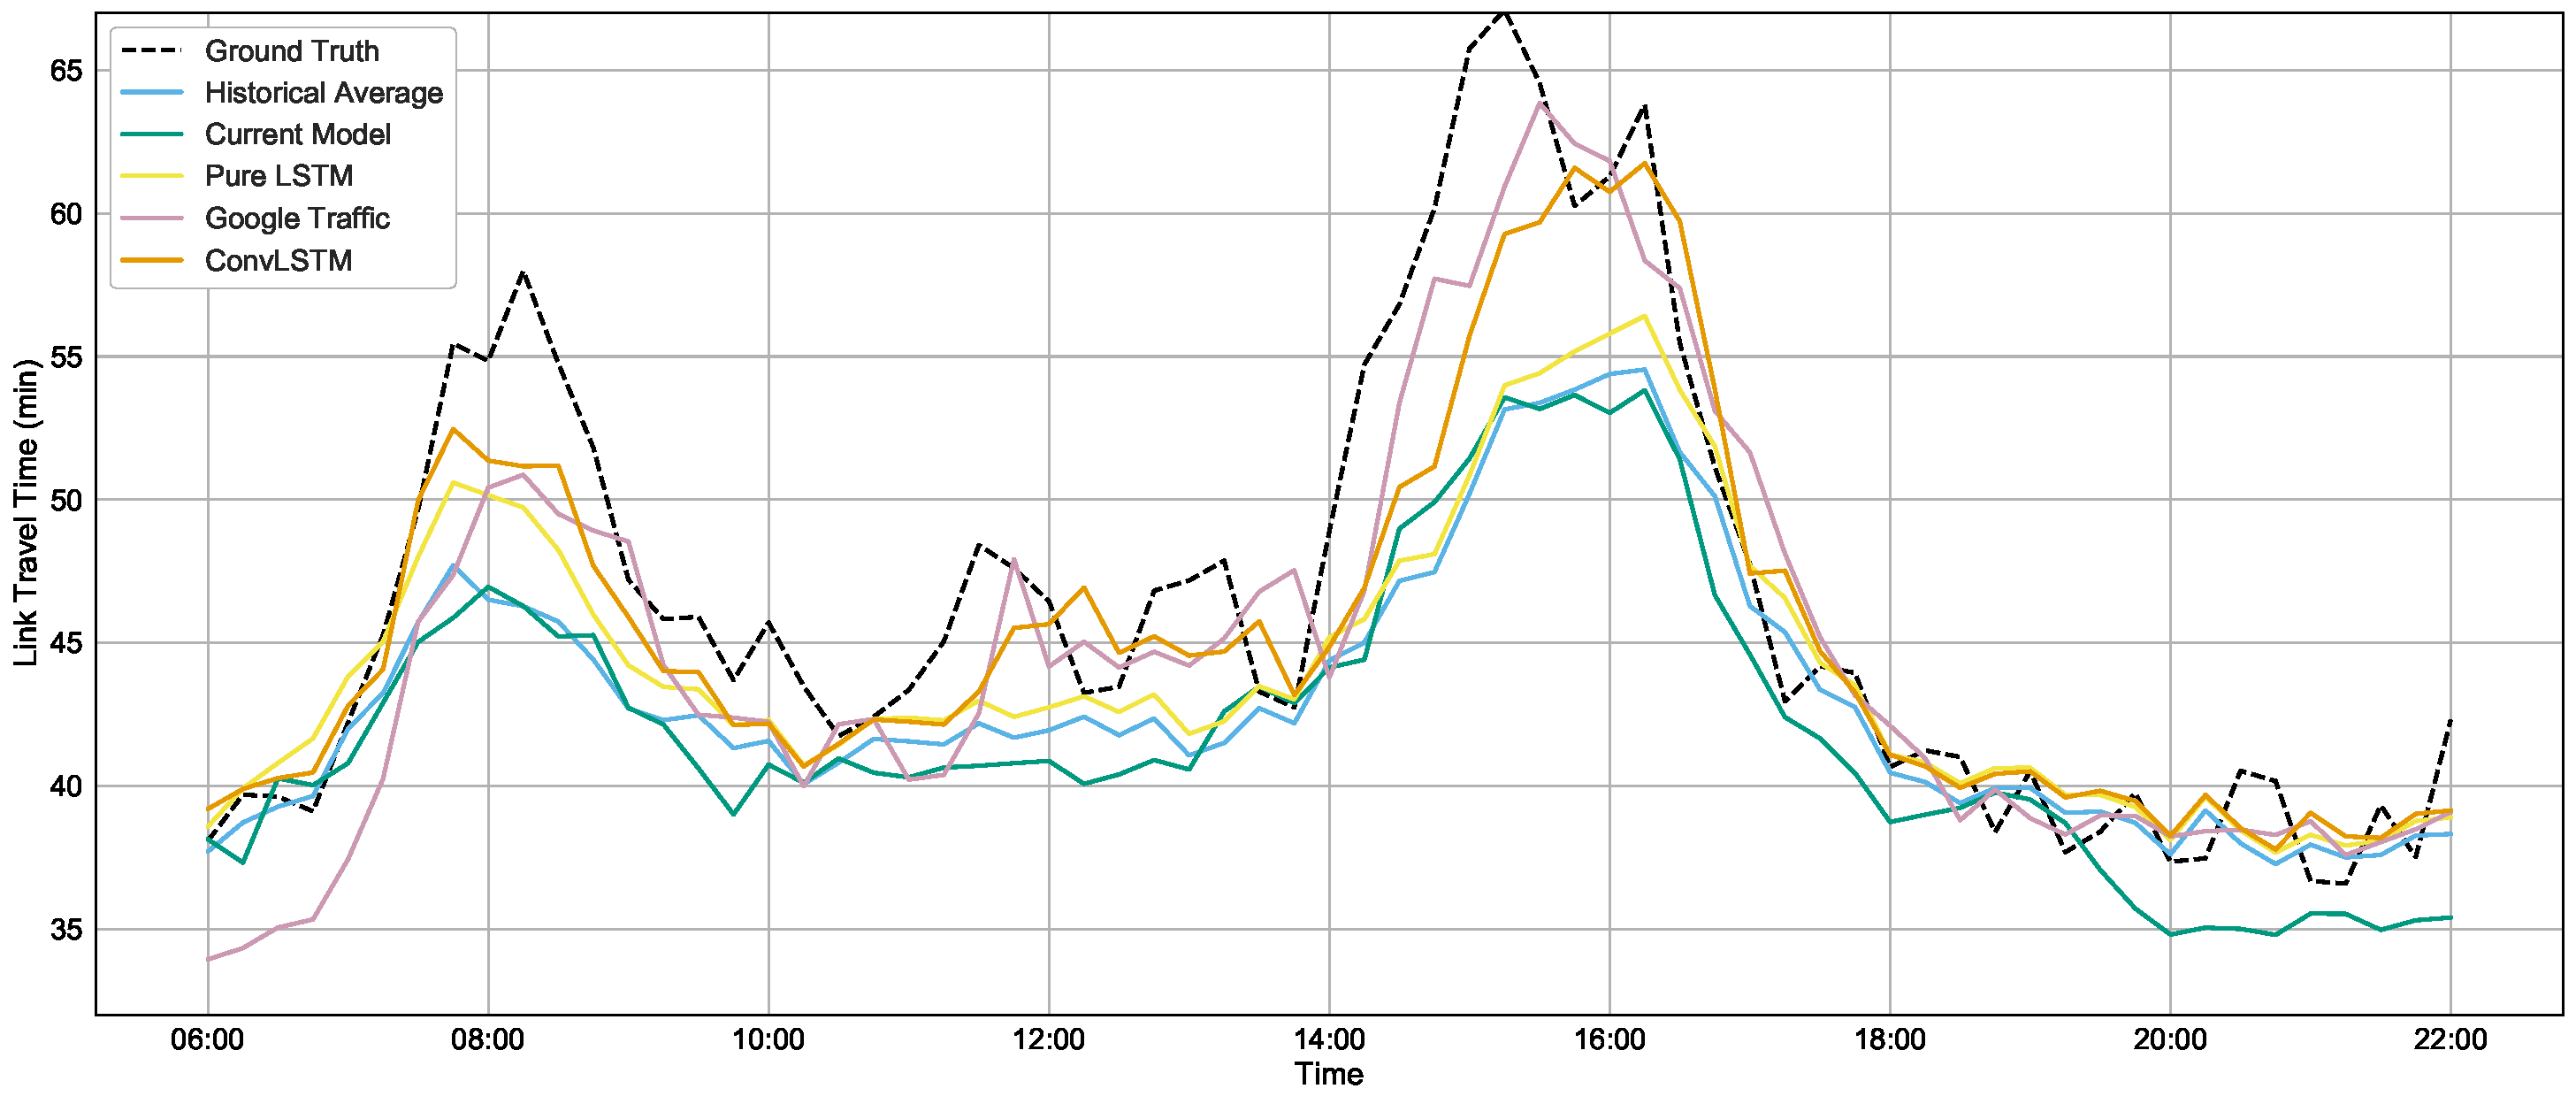
\includegraphics[width=\textwidth]{plots/comparison_day.pdf}
  \caption{}
  \label{fig:comparison_day}
\end{figure*}
\begin{figure*}
  \centering
  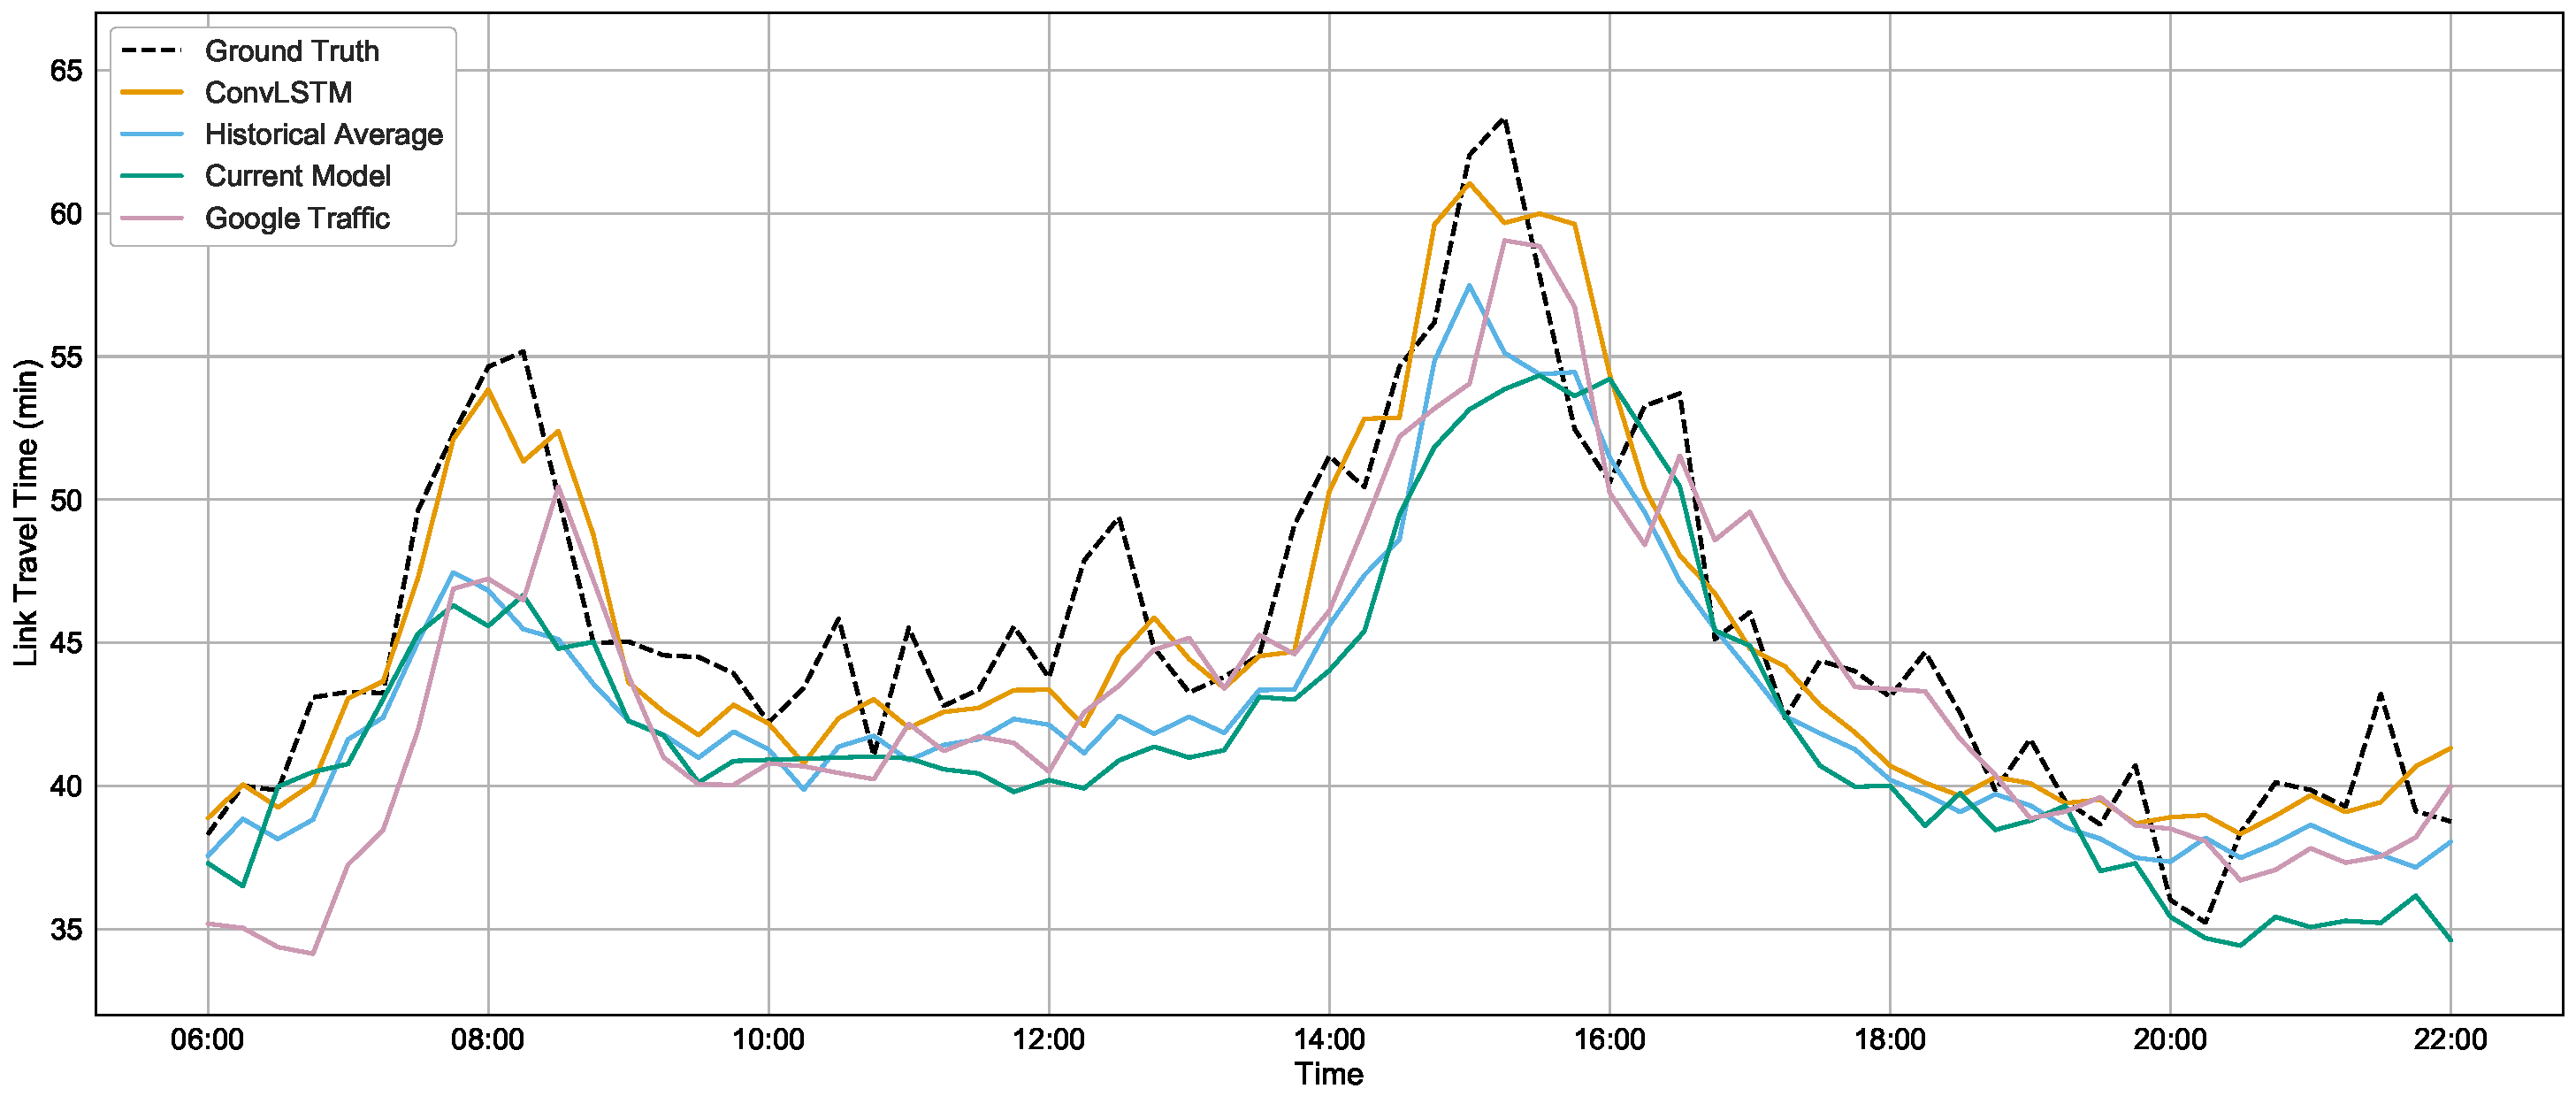
\includegraphics[width=\textwidth]{plots/comparison_day_2.pdf}
  \caption{}
  \label{fig:comparison_day_2}
\end{figure*}


\subsection{Comparison}
We compare the performance of the proposed \emph{ConvLSTM} model for bus link travel time prediction against the presented baseline models. The overall results from \Cref{tab:results} shows that the \emph{ConvLSTM} model outperforms the other methods. The \emph{current model} performs the worst, even compared to the \emph{historical average} model, on which it is based. This is most likely due to the rule-based enforcement of recovery from delays, even though the data weights against a recovery.

Although the advantage might seem small it is emphasized that evaluation measurements are averaging their response, and thus the increased accuracy can be much higher on individual journeys, especially if they experience very irregular travel times. To investigate this, we focus our analysis on periods when the transport system is most vulnerable, and even small changes in regularity can propagate, since recovery is not an option, i.e.\ morning and afternoon peeks.

\begin{table}[!ht]
  \center
  \begin{tabular}{l|rrr}
  Model &  RMSE &  MAE &  MAPE \\
  \hline
  \hline
  Historical Average &        6.40 &       5.57 &     10.62 \% \\ \hline
  Current Model      &        6.69 &       5.88 &     11.22 \% \\ \hline
  Pure LSTM          &        0.00 &       0.00 &      0.00 \% \\ \hline
  Google Traffic     &        5.25 &       4.62 &      9.17 \% \\ \hline
  ConvLSTM           &        2.64 &       2.09 &      4.04 \% \\ \hline
  \end{tabular}
  \caption{Results: Morning peek (7--9)}
  \label{tab:morning_peek}
  
\end{table}

\begin{table}[!ht]
  \center
  \begin{tabular}{l|rrr}
  Model &  RMSE &  MAE &  MAPE \\
  \hline
  \hline
  Historical Average &    5.90 &   4.65 &  8.28 \% \\ \hline
  Current Model      &    6.28 &   5.20 &  9.37 \% \\ \hline
  Pure LSTM          &    0.00 &   0.00 &  0.00 \% \\ \hline
  Google Traffic     &    4.16 &   3.34 &  6.21 \% \\ \hline
  ConvLSTM           &    3.79 &   3.02 &  5.61 \% \\ \hline
  \end{tabular}
  \caption{Results: Afternoon peek (14--18)}
  \label{tab:afternoon_peek}  
\end{table}

\Cref{tab:morning_peek} and \Cref{tab:afternoon_peek} shows the evaluation results for \emph{morning peeks (weekdays, 7--9)} and \emph{afternoon peeks (weekdays, 14--18)} respectively for the time-step $t + 1$.

The peek hour evaluation shows that the \emph{ConvLSTM} model increases its performance over the baseline models when the transport network is put under stress. In the morning peek, the \emph{ConvLSTM} model performs similar as the overall, whereas the baseline models all experience decreased performance of up to several minutes in both the RMSE and MAE, and an increased MAPE of roughly one third. 

Likewise the afternoon peek evaluation shows improvements with respect to the baseline models, even though the \emph{ConvLSTM} model also decreases its performance compared to the overall results. The outperformance is neither as significant as in the morning peek, and as the \emph{Google Traffic} model also performs quite well leaving the gap less than a minute. 

The get a little more detailed view of how the different models perform on the micro-level (i.e.\ the specific journey) we can inspect a single day of predictions. A random weekday from the test-dataset is plotted in~\Cref{fig:comparison_day}, which shows the accumulated travel time of all 32 links and the predicted travel time at time-step $t + 1$ both for the proposed and baseline models.

In this particular day (a Thursday) the peek hour traffic was worse than normal, which leads both the \emph{historic averaging} model and the \emph{current model} to both underestimate travel time in the peek periods. Remember that the \emph{current model} is based on the \emph{historic averaging} model, so it is not unexpected that they perform very similar. There is also an small peek in travel time in the midday hours, which none of these historic averaging models are able to predict.

On the other hand, both the \emph{Google Traffic} model and the proposed \emph{ConvLSTM} model get much closer to the ground truth in the peek ours. The \emph{Google Traffic} model seems to predict more accurate then \emph{ConvLSTM} model in the afternoon peek, whereas the opposite occurs in the morning peek. Even more interesting is the detection of the irregular peek in the midday hours, which both the \emph{Google Traffic} model and the proposed \emph{ConvLSTM} model are able to adjust to, at least to some degree.

\Cref{fig:comparison_day_2}~shows another example (a Friday). Here the difference between the proposed model and the historical averaging and current model baselines are a bit weaker, simply because the the day to a larger degree follows the average pattern for a Friday (especially around the afternoon peek). Even though, the proposed model still performs the best, and it also supports the claim, that the proposed model is strongest when the traffic pattern deviates from the normal pattern, i.e. when the transport network is under stress.

\section{Conclusion}
\label{sec:conclusion}
This paper has proposed a multi-output, multi-time-step deep neural network for bus travel time prediction using Convolutional and Long short-term memory (LSTM) layers. Results show, that the proposed model network outperforms other popular and recent methods. This includes Google's Traffic model based on crowd-sourced live data, and the current model deployed by Movia, the public transport authority in the Greater Copenhagen Area.

For the prediction accuracy to be increased further it is proposed to apply ensemble/multi-model approaches. In this case the proposed model can be included and used as a sub-model for the ensemble. Further research should be invested in the more rare, but highly impacting deviations, e.g.\ traffic incidents, extreme weather conditions, etc.

\section*{References}
\bibliographystyle{elsarticle-num-names}
%\bibliography{../references/library}
\bibliography{c:/development/references/library}

\end{document}